\subsection{Contexto da pesquisa} \label{subsec:contexto}
\citeonline{mateus} A necessidade de desenvolvimento do planejamento estratégico no mundo corporativo e no dia-a-dia torna a análise de séries temporais e previsões valiosas ferramentas para apoiar o processo de tomada de decisão a curto, médio e longo prazo. Devido a não linearidades, sazonalidade, tendência e ciclicidade nos dados temporais, o desenvolvimento de modelos de previsão eficientes é uma tarefa desafiadora. 

No conjunto de dados da SANEPAR, há um volume significativo no consumo de água e, com a interrupção que a cidade sofreu, é necessário avaliar os dados para ter certeza do que está acontecendo quando a interrupção e os picos de água ocorrem entre horas e dias.

Entre os modelos preditivos que serão apresentados em uma revisão sistemática, avalie o melhor modelo que pode ser usado e valide quando e como ocorrerá a escassez de água. Essas análises serão feitas em \textit{python}.
Explorando o que são séries temporais e aprendizado de máquina. As séries temporais são dados armazenados ao longo do tempo que permitem que um observador analise as anomalias nos dados. Nas séries temporais, a classificação dos dados por ano ou dia é fundamental e, se os dados forem atribuídos aleatoriamente, pode ser mais difícil prever e tomar decisões com base nos dados coletados. 
A análise das médias pode ser bastante perigosa se você não excluir pontos fora da curva também conhecidos como ``\textit{outliers}''. Isto pode gerar dados muito positivos ou negativos que não correspondem à realidade.
 
 
\begin{figure}[H]
	\centering
	\caption{Paradigma de aprendizado de máquina}
	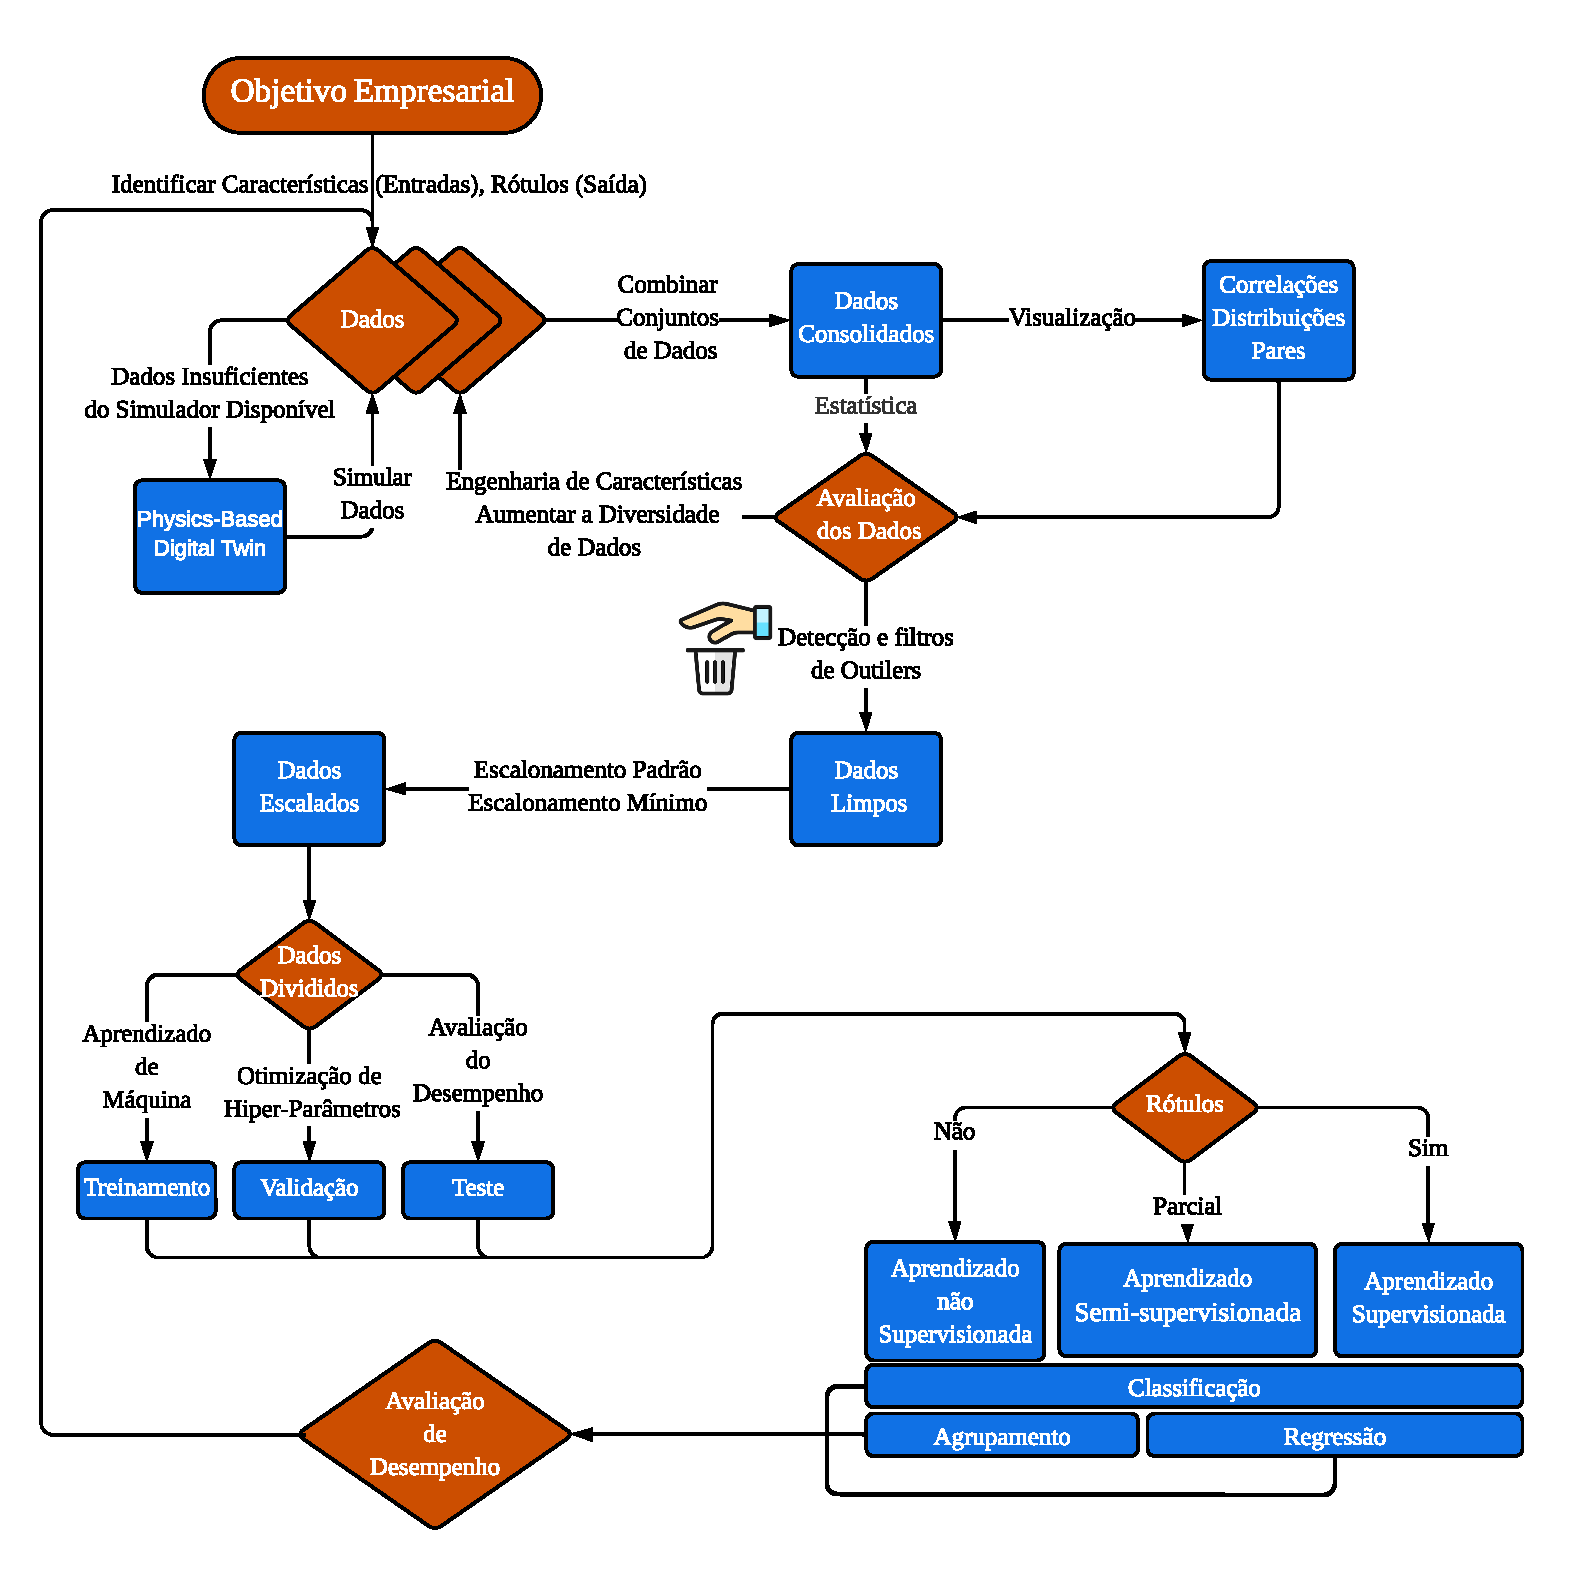
\includegraphics[width=1\linewidth]{Introducao/Figuras/paradigma-ml}
	
	Fonte: Elaboração própria
	\label{fig:paradigma-ml}
\end{figure}
  
      
\subsubsection{Motiva\c c\~ao da pesquisa} \label{subsubsec:motivacao}
   %Escrever algo motivador 
    
    De acordo com \cite{vasconcelos_2020} Curitiba e região metropolitana enfrentou um rodízio com $36$ horas com água e $36$ horas sem abastecimento. A média geral dos reservatórios da região está em $27,96\%$ da capacidade. Assim em medida a isso essa pesquisa tem como a abordagem da falta de água, essa falta que pode ser vista como uma seca, em média nos anos anteriores de 2020 a chuva tem marcado a quantia de $1.704$ mm. \cite{vasconcelos_2020} Desde 2016, quando registrou 1.704 mm de chuva, Curitiba não atingiu mais a média anual de precipitação, que é de 1.490 mm, com base em dados da estação pluviométrica do IBMET.  Apesar de abaixo da média, o mínimo registrado desde então ocorreu em 2020, com 1.158 mm.
    
    Em meio a essa motivação, pode-se interpretar melhor os dados que a SANPEAR ofereceu para prever e evitar a escassez de água que foi registrada e a anomalia que foi detectada em 2020 com o retorno das chuvas, os reservatórios aumentaram de nível.
    
    